\documentclass[a4paper, 12pt, onepage]{article}
\usepackage[utf8]{inputenc}
\usepackage[russian]{babel}
\usepackage{fullpage}
\usepackage{indentfirst}
\usepackage{graphicx}
\usepackage{cmap}
\usepackage{amsmath}
\usepackage{amssymb}
%\usepackage{pdfpages}
\usepackage{tikz}

\usepackage[pdftex, unicode, pdfstartview=FitH, colorlinks, linkcolor=black, citecolor=blue, urlcolor=blue]{hyperref}
\usepackage{url}
\def\UrlFont{\rmfamily}

\usepackage{setspace}
\onehalfspacing

\usepackage{cyrtimes}
\renewcommand\ttdefault{cmtt}

\frenchspacing
\sloppy
\selectlanguage{russian}

\begin{document}

\author{Красильников Иван}
\title{Задание 5}
\maketitle

\subsection*{Задача 1}
Я реализовал метод конформных предикторов с использованием Python:
{
\footnotesize
\begin{verbatim}
import numpy

def conformal_algorithm(train_points, test_point):
    # построение многочлена f(x)=a+bx+cx^2 по обучающей выборке включая
    # проверяемую точку
    xs = [x for (x, y) in train_points] + [test_point[0]]
    ys = [y for (x, y) in train_points] + [test_point[1]]
    N = len(xs)
    c, b, a = numpy.polyfit(xs, ys, 2)

    # вычисление меры странности - отклонения y от f(x)=a+bx+cx^2
    arr = []
    for i in range(N):
        x, y = xs[i], ys[i]
        arr.append([abs(a + b*x + c*x*x - y), i])

    arr.sort()

    for new_index, (value, old_index) in enumerate(arr):
        if old_index == N - 1:
            return (new_index + 1) / float(N)

sample_x = [-1.0, -0.75, -0.5, -0.25, 0.25, 0.75, 1.0]
sample_y = [1.0, 0.75, 0.5, 0.25, 0.25, 0.75, 1.0]
sample = zip(sample_x, sample_y)

c, b, a = numpy.polyfit(sample_x, sample_y, 2)
print a  # точечное предсказание в x=0

for i in range(5000):
    y = i / 10000.0
    p = conformal_algorithm(sample, (0.0, y))
    if p <= 0.95:
        print y,   # значения в доверительном интервале
\end{verbatim}
}

Метод наименьших квадратов подгоняет под обучающую выборку следующий квадратный многочлен:
$$ f(x) = 0.2483 - 0.0078x + 0.7879x^2, $$
Таким образом, точечное предсказание в $x=0$ равно $0.2483$.

Значения уверенности в каждом значении $y$, построенные методом конформных
предикторов по сетке с шагом $0.0001$ приведены на следующем рисунке:
\begin{figure}[h]
  \centering
  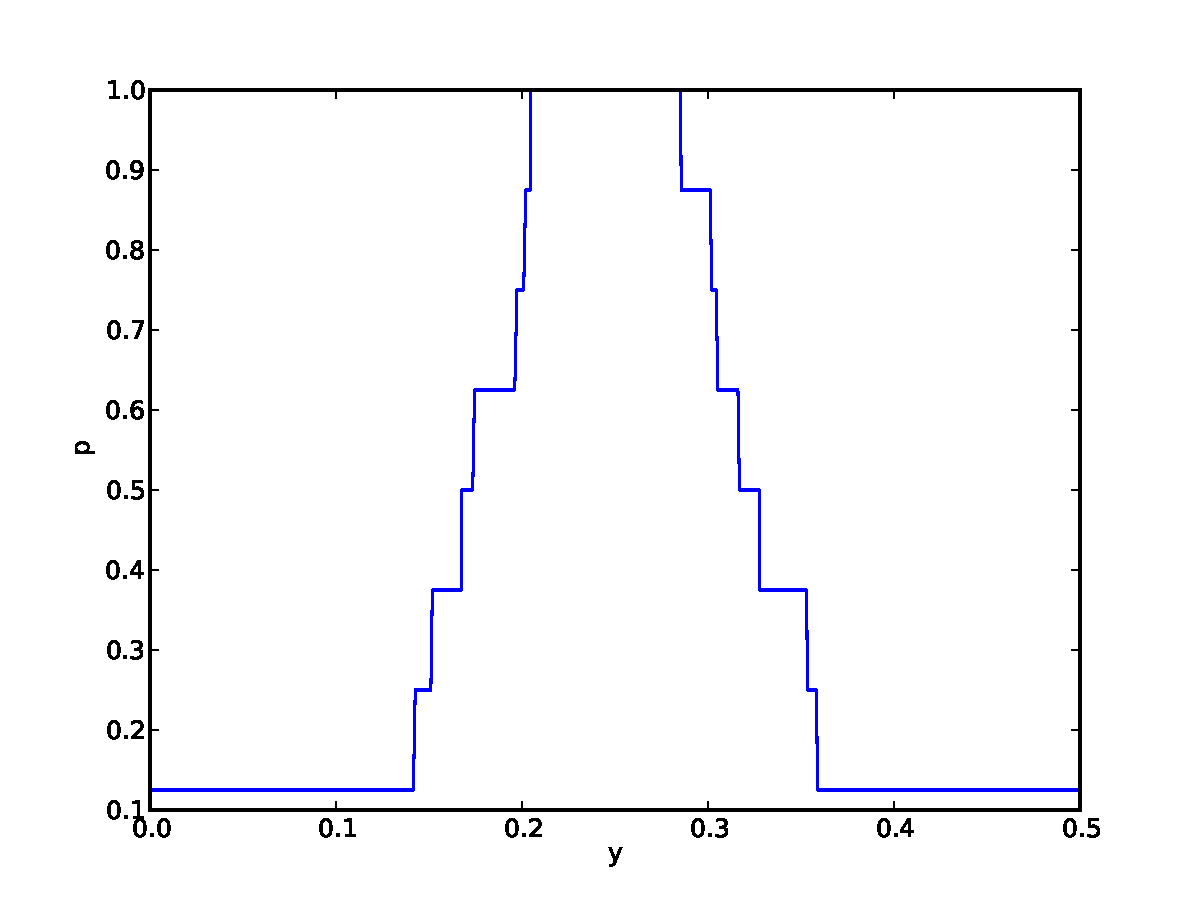
\includegraphics[scale=0.7]{figure2.pdf}
\end{figure}

Доверительный интервал для уровня толерантности $p=0.95$ образуют
значения $y$ в интервале $[0.1426, 0.3588]$.

\newpage
\subsection*{Задача 3}

Я буду использовать обозначение $[P]$ для индикаторных функций: $[P] = 1$, если предикат (условие) $P$ выполняется,
и $[P] = 0$ иначе.

\textbf{3.1.} Необходимо сделать дополнительные предположения в этой задаче.
Если $u(x)$ -- произвольный многочлен $n-1$ степени, то искомое решение $f(x) = u^{(n)}(x) = 0$,
подставляя его в интегральное уравнение получим, что $u(x)$ должен быть равен нулю.
Чтобы разрешить это противоречие, я буду предполагать, что нам дана
функция $u(x)$, у которой $u(0) = 0$, $u'(0) = 0$, $\ldots$, $u^{(n-1)}(0) = 0$.

Из матанализа известно следующее свойство производных:
$u(x) - u(0) = \int_0^x u'(t) dt$. Воспользуемся им несколько раз:

\begin{align*}
  u(x) &= \int_0^x u'(t) dt
        = \framebox{$\displaystyle \int_0^1 [t \leqslant x] u'(t) \,dt$}
        = \int_0^1 [t \leqslant x] \int_0^t u''(s) \,ds\, dt \\
       &= \int_0^1 [t \leqslant x] \int_0^1 [s \leqslant t] u''(s) \,ds\, dt
        = \int_0^1 \int_0^1 [s \leqslant t \leqslant x] u''(s) \,ds\, dt \\
       &= \int_0^1 [s \leqslant x] \left(\int_0^1 [s \leqslant t \leqslant x] \,dt\right) u''(s) \,ds
        = \framebox{$\displaystyle \int_0^1 [s \leqslant x] (x - s) u''(s) \,ds$} \\
       &= \int_0^1 [s \leqslant x] (x - s) \left(\int_0^1 [t \leqslant s] u'''(t) \,dt\right)\, ds
        = \int_0^1 \int_0^1 [t \leqslant s \leqslant x] (x - s) u'''(t) \,dt\, ds \\
       &= \int_0^1 [t \leqslant x] \left(\int_t^x (x - s) ds\right) u'''(t) \,dt
        = \framebox{$\displaystyle \int_0^1 [t \leqslant x] \frac12 (t^2 - 2tx + x^2) u'''(t) \,dt$} = \ldots
\end{align*}

Таким образом, уже наблюдается закономерность, и получаются следующие
ядра $K_n(x, t)$ для $n$-х производных:
\begin{align*}
  K_1(x, t) &= [t \leqslant x], \\
  K_2(x, t) &= [t \leqslant x] (x - t), \\
  K_3(x, t) &= [t \leqslant x] \frac12 (t^2 - 2tx + x^2), \\
  \ldots  \\
  K_n(x, t) &= [t \leqslant x] \int_t^x K_{n-1}(x, s) \, ds.
\end{align*}

\textbf{3.2.} Рассмотрим случай, когда $n=1$.
Возьмем $u_k(x) = \frac1k \sin(kx)$. Заметим, что для неё выполняется потребованное выше условие о том, что $u(0)=0$.
Очевидно, что $\lim_{k\to\infty} \sup_x |u_k(x)| = 0$, но
$\lim_{k\to\infty} \sup_x |u'_k(x)| = \lim_{k\to\infty} \sup_x |\cos(kx)| = 1.$
Поэтому решение интегрального уравнения из пункта 1 будет неустойчиво.

\textbf{3.3.} Модифицируем интегральное уравнение следующим образом. Будем искать решение $f^*(x)$ в некотором классе
функций (непрерывных, например), которое доставляет минимум функционалу:
$$H(f) = \sup_{x \in [0, 1]} \left|\int_0^1 K(x, t) f(t) \, dt - u(x)\right| + \sup_{x \in [0, 1]} |f(x)|. $$

Если $\sup_x |u(x)| \leqslant \varepsilon$, то для $f(x) = 0$, $H(f) \leqslant \varepsilon \to 0$ при $\varepsilon \to 0$.
А для любого решения $f(x)$, такого что $\sup_x |f(x)| = s > 0$, $H(f) \geqslant s$ и не стремится к нулю.
А значит при $\varepsilon < s$ все такие решения будут отброшены в пользу решений, более близких к нулевому.
То есть будет выполняться $\sup_x |f^*(x)| \to 0$ при $\varepsilon \to 0$.


\end{document}
